\tocless\subsection{Objective}
In this experiment, it was decided to look into how scaling down the size of the image would influence its classification. Three images were scaled down to 10\% of their size for this purpose, Figure \ref{fig:bananaPreRes}, Figure \ref{fig:apple_piePreRes} and Figure \ref{fig:pizzaPreRes}. Each of these images were run through the model before and after image resizing and the predictions were recorded.

\begin{figure}[h]
	\centering
    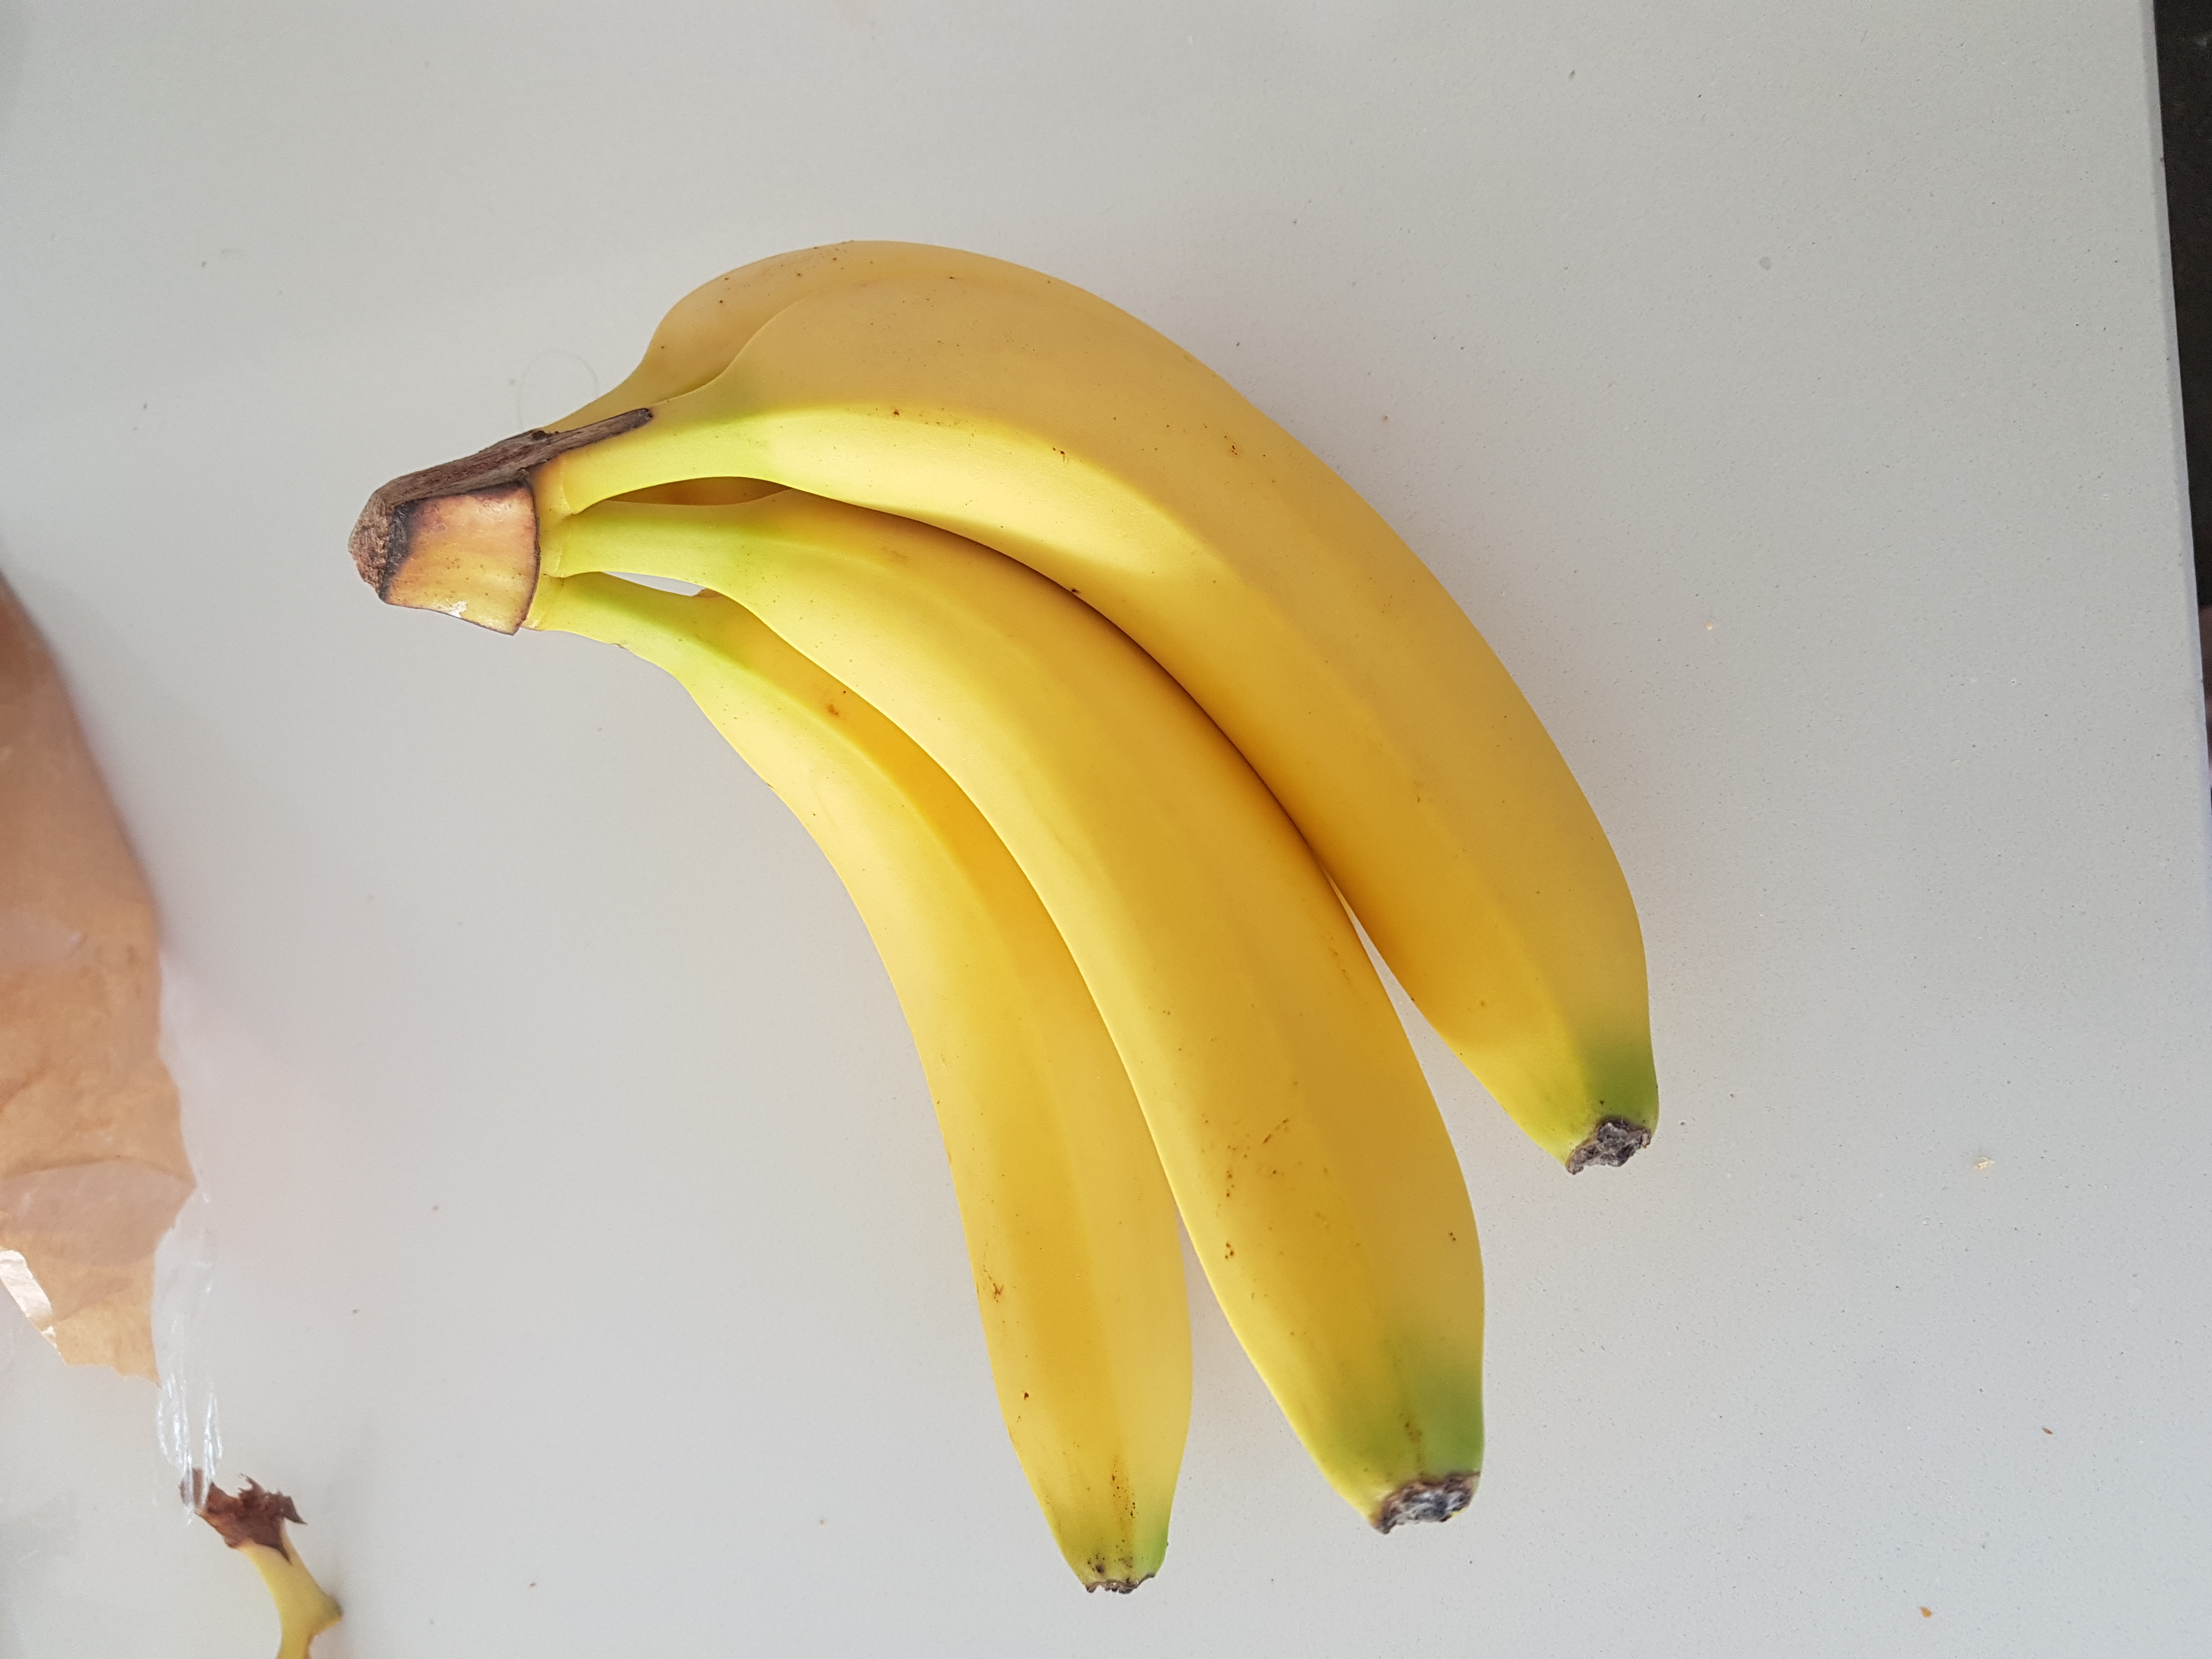
\includegraphics[scale=0.05]{banana1}
    \caption{Banana Image Pre-Resolution}
    \label{fig:bananaPreRes}
\end{figure}

\begin{figure}[h]
	\centering
    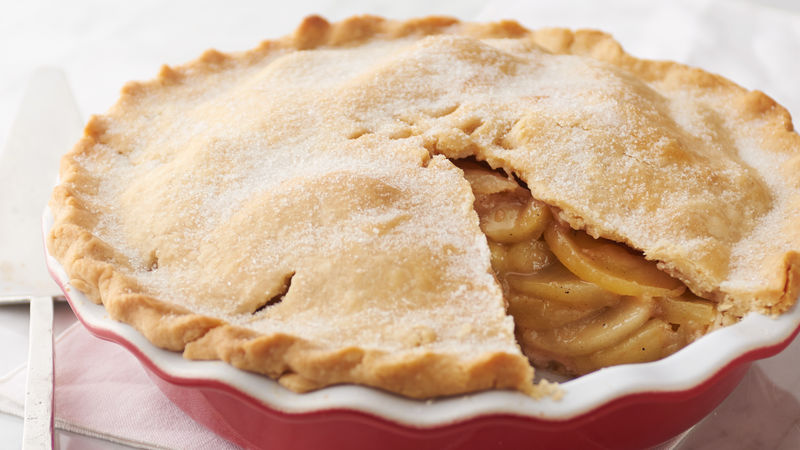
\includegraphics{apple_pie}
    \caption{Apple Pie - sourced from https://www.bettycrocker.com/}
    \label{fig:apple_piePreRes}
\end{figure}

\begin{figure}[h]
	\centering
    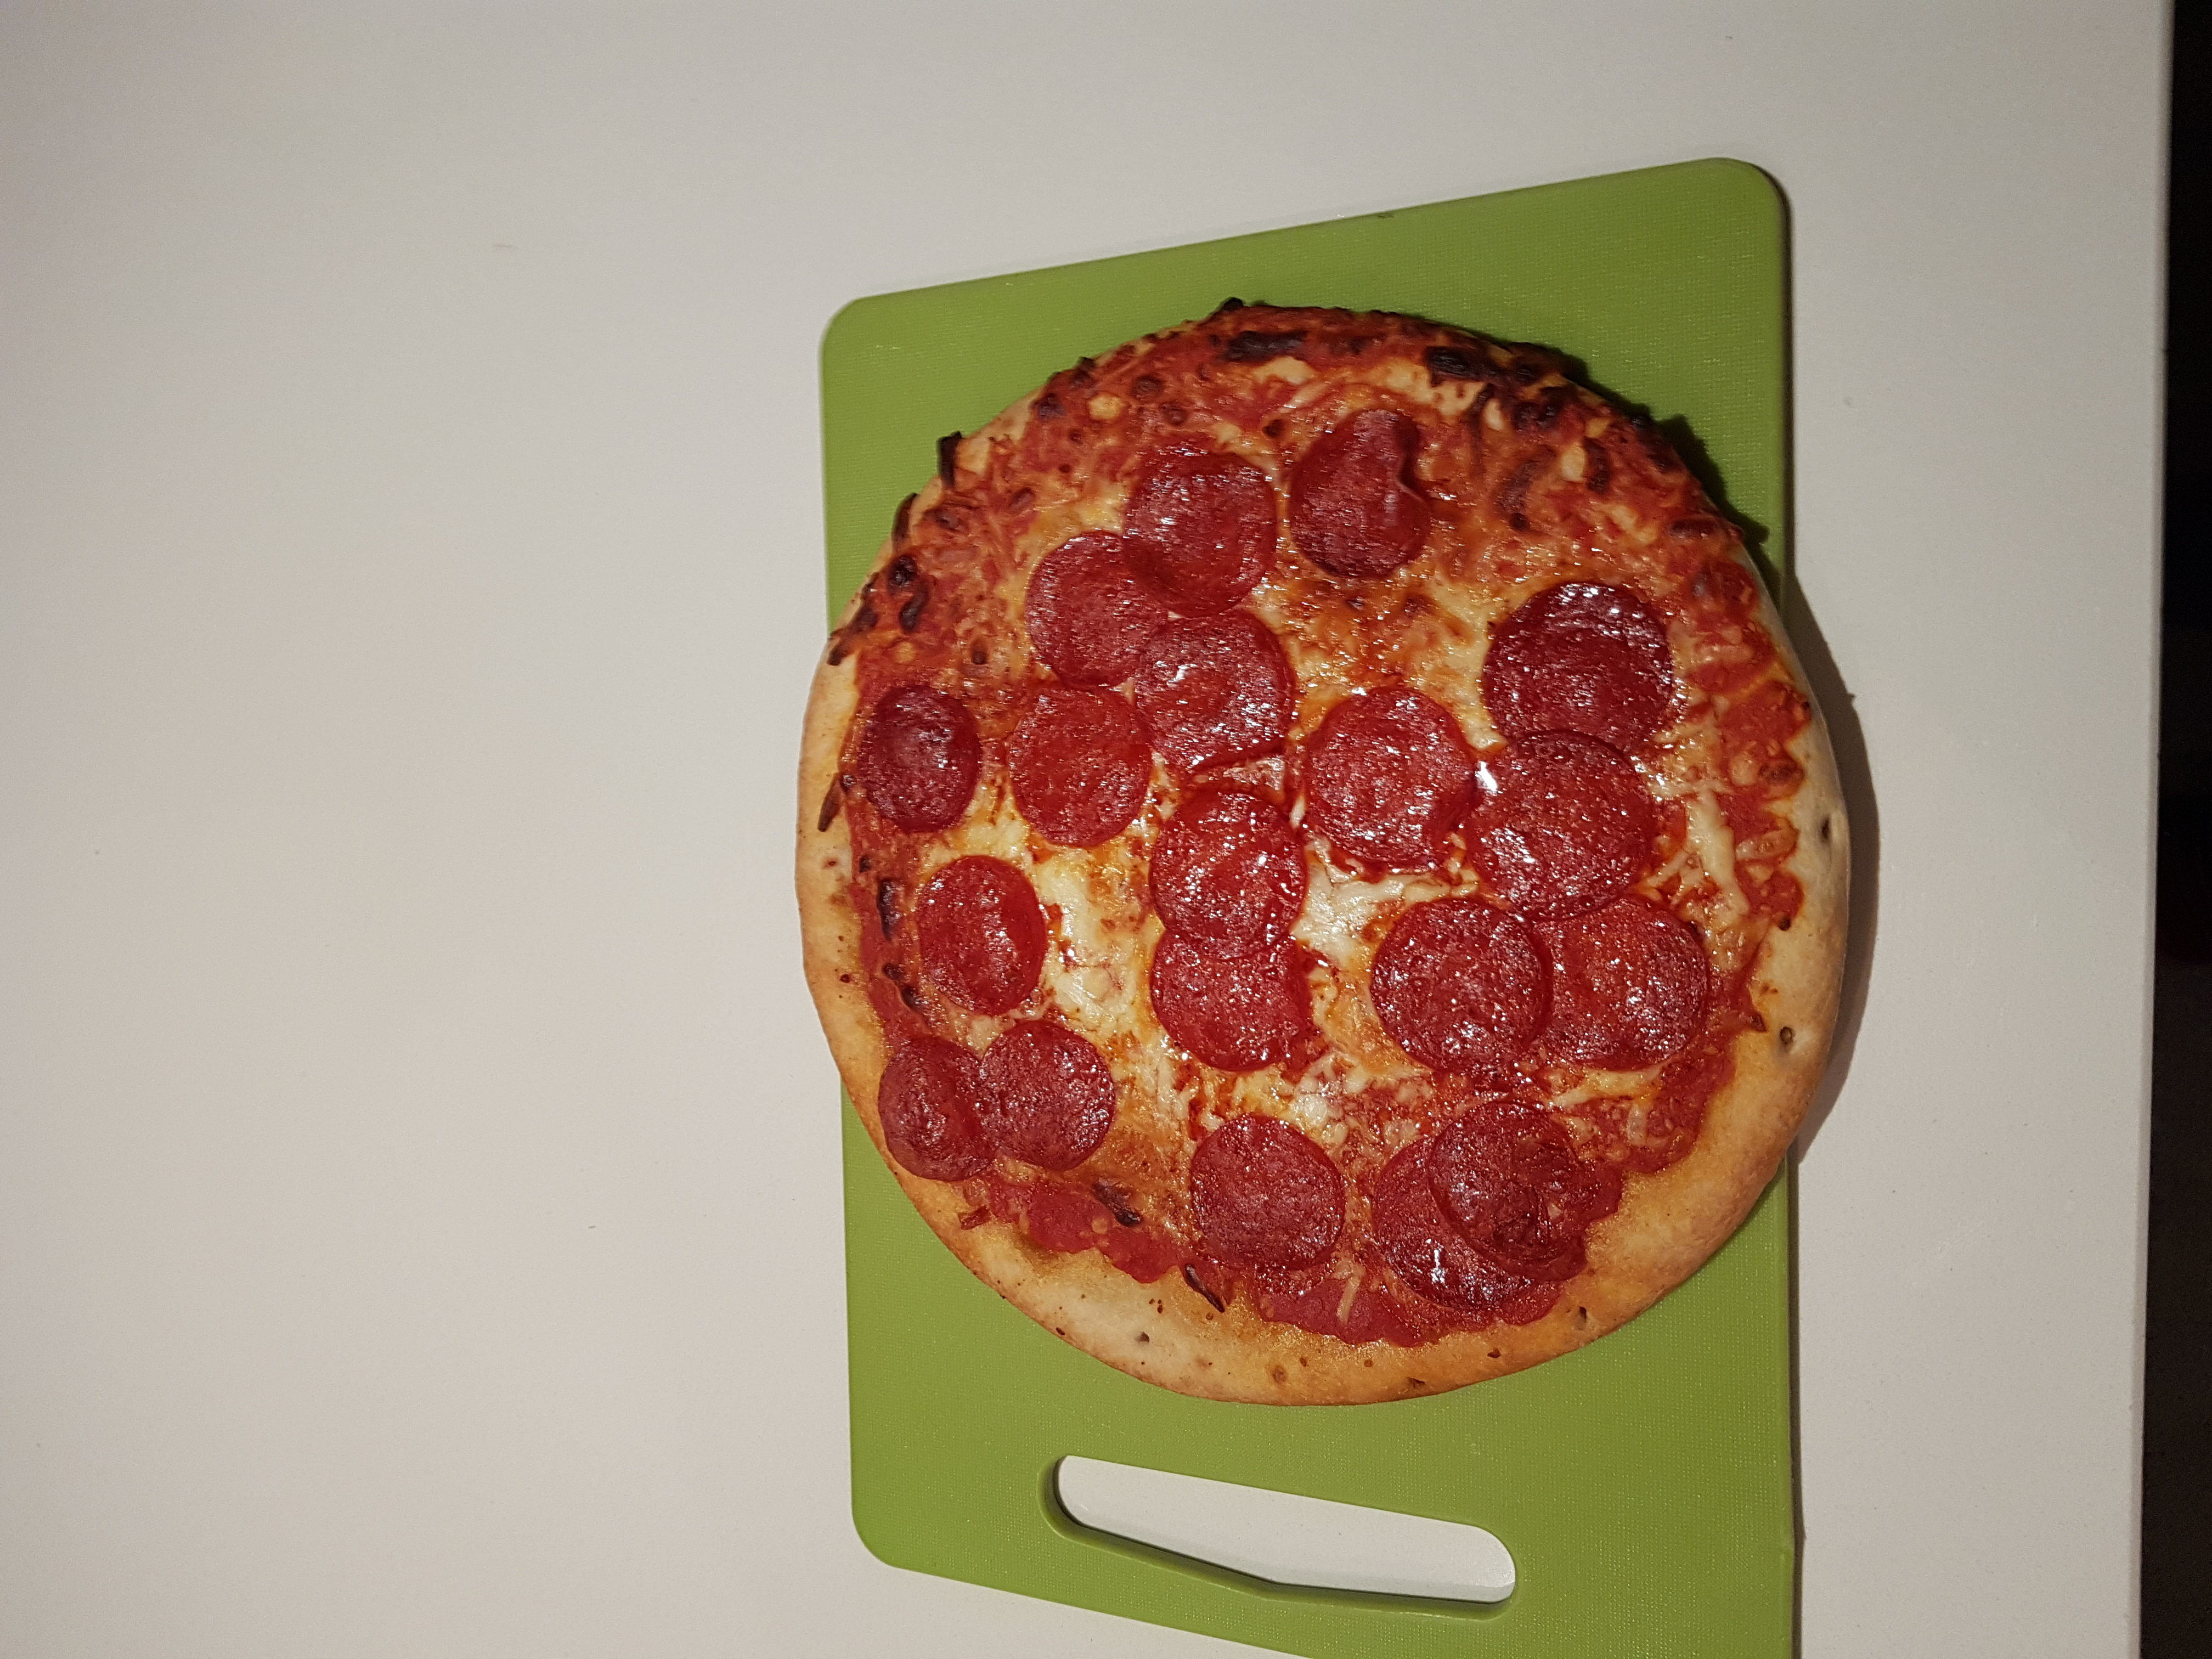
\includegraphics[scale=0.05]{pizza1}
    \caption{Pizza Image Pre-Resolution}
    \label{fig:pizzaPreRes}
\end{figure}

\tocless\subsection{Results}
The results of the images before and after were somewhat contrasting as seen in Table \ref{scaledImages}.
The 'Top 1' notation in the table suggests that the food was predicted as the number one prediction. The decimal value is the probability of that food type being the correct classification.

\begin{table}[]
\centering
\caption{Results of Down Scaled Images}
\label{scaledImages}
\begin{tabular}{|l|l|l|}
\hline
\textbf{Food Image}& \textbf{Pre-Scaled Image} & \textbf{Scaled Image}   \\ \hline
Banana     & Top 1 : 0.9971   & Top 1 : 0.9995 \\ \hline
Apple Pie  & Top 1 : 0.7986   & Top 5 : 0.0836 \\ \hline
Pizza      & Top 1 : 0.9753   & Top 1 : 0.9705 \\ \hline
\end{tabular}
\end{table}

\tocless\subsection{Analysis}
As we can see in Table \ref{scaledImages}, the banana (Figure \ref{fig:bananaPreRes}) has a very similar prediction and probability.
This would indicate that the classifier does not need clear quality images for bananas but maybe shape, texture and colour are important factors.

The apple pie (Figure \ref{fig:apple_piePreRes}) has drastically different results in Table \ref{scaledImages}.
Originally the apple pie was correctly predicted with a probability of 0.7986 but after downscaling, the apple pie was the fifth food predicted with a likelihood of 0.0836.

The image of the pizza (Figure \ref{fig:pizzaPreRes}), had very similar results before and after resizing.
This might indicate that pizza is determined more by shape, texture and colour that fine quality.


